% tipo di documento
\documentclass[a4paper, twoside, openright]{report}
% codifica caratteri
\usepackage[utf8]{inputenc}
% encoding del testo
\usepackage[T1]{fontenc}
% dimensione dei margini
\usepackage[a4paper,top=2.5cm,bottom=2.5cm,left=3cm,right=3cm]{geometry}
% dimensione del font
\usepackage[fontsize=12pt]{scrextend}
% lingua del testo
\usepackage[english,italian]{babel}
% package per generare testo fittizio. Potrebbe essere
% utile nel controllare quanto un capitolo potrebbe essere
% grande e quindi quanto occupa nella pagina
\usepackage{lipsum}
% per ruotare le immagini
\usepackage{rotating}
% per modificare l'header delle pagine 
\usepackage{fancyhdr}
% per allineare in modo giustificato
\usepackage{ragged2e}
\justifying
% uso delle immagini
\usepackage{graphicx}
\usepackage{float}
% uso dei colori
\usepackage[dvipsnames, table]{xcolor}         
% uso dei listing per il codice
\usepackage{listings}          
% per inserire gli hyperlinks tra i vari elementi del testo 
\usepackage[colorlinks=true, allcolors=black]{hyperref}    
% diversi tipi di sottolineature
\usepackage[normalem]{ulem}
% package e comando per creare pagine vuote
\usepackage{afterpage}
\newcommand\blankpage{%
    \null
    \thispagestyle{empty}%
    \addtocounter{page}{-1}%
    \newpage
}
    
% package per creare comandi personalizzati
\usepackage{xpatch}
% package helper per le liste puntate
\usepackage{enumitem}
% package per l'utilizzo dei colori
% package per l'highlighting del codice
\usepackage{minted} %(non funziona sotto windows)
% package per gestire le caption 
\usepackage{caption}
\usepackage{subcaption}
% per gestire tabelle su più pagine
\usepackage{longtable}
% per combinare le righe di una tabella
\usepackage{multirow}
% per creare i tree di directory
\usepackage{dirtree}
%per i todo
\usepackage{todonotes}

% per le icone a fianco dei titoli di sezione
\usepackage{etoolbox}
\newcommand{\icon}[1]{\includegraphics[height=12pt]{#1}}
\robustify{\icon}

%bibliografia con biber
\usepackage[
backend=biber,
style=alphabetic,
sorting=ynt
]{biblatex}
\addbibresource{Bibliography.bib}
\usepackage{csquotes}

% -----------------------------------------------------------------

% Modifica lo stile dell'header
\pagestyle{fancy}
\fancyhf{}
\lhead{\rightmark}
\rhead{\textbf{\thepage}}
\fancyfoot{}
\setlength{\headheight}{15pt}

% Rimuove il numero di pagina all'inizio dei capitoli
\fancypagestyle{plain}{
  \fancyfoot{}
  \fancyhead{}
  \renewcommand{\headrulewidth}{0pt}
}

% comandi per cambiare temporaneamente la lingua
% abstract in inglese, al fine di cambiarne il titolo
\xpretocmd{\abstract}{\selectlanguage{english}}{}{} 
\xapptocmd{\endabstract}{\selectlanguage{italian}}{}{}

% formattazione e highlight del codice
\usemintedstyle{manni}

% rimozione del prefix per le tabelle
\captionsetup[table]{labelformat=empty}

% environment per impostare il codice in piu' pagine
\newenvironment{code}{\captionsetup{type=listing}}{\hfill\break}

% imposta la "profondità" delle sezioni che devono essere numerate (secnumdepth) o mostrate nell'indice (tocdepth). 3 è subsubsection
\setcounter{secnumdepth}{3}
\setcounter{tocdepth}{3}

% -----------------------------------------------------------------
\begin{document}
\begin{titlepage}

\begin{center}
    \textbf{\huge{Università degli Studi di Torino}}
    \vspace{2mm}
    \\ \LARGE{Dipartimento di informatica}
    \vspace{5mm}
    \\ 
\includegraphics[keepaspectratio=true,scale=0.4]{images/unito_logo.png}
    \vspace{5mm}
\end{center}

\begin{center}
    \LARGE{Tesi di Laurea Magistrale in Informatica} 
\end{center}

\vspace{15mm}
\begin{center}
    \textbf{\huge{ Progetto Velocity }}
\end{center}
\vspace{30mm}

\begin{minipage}[t]{0.47\textwidth}
	{\large{Relatore:}{\normalsize\vspace{3mm}
	\bf\\ \large{Petrone Giovanna} \normalsize\vspace{3mm}\bf}}
\end{minipage}
\hfill
\begin{minipage}[t]{0.47\textwidth}\raggedleft
	{\large{Candidato:}{\normalsize\vspace{3mm} \bf\\ \large{Dentis Lorenzo} \\ \small{Matricola 914833}}}
\end{minipage}

\vspace{40 mm}
\hrulefill
\\ \centering{\large{ANNO ACCADEMICO 2023/2024}}

\end{titlepage}
\thispagestyle{plain}

\vspace*{\fill}
Prima di procedere con la trattazione, vorrei ringraziare tutte le persone senza le quali non sarei mai arrivato qui.
Un grazie va ai miei genitori, che mi hanno sempre sostenuto nel mio percorso di studi. 
Il loro supporto mi ha sempre permesso di studiare ciò che mi piaceva e di perseguire i miei obiettivi, senza preoccuparmi di null'altro che non fosse il mio percorso di studi.
Ringrazio tutti i colleghi che ho incontrato durante il mio percorso di studi, per i momenti di svago ma soprattutto per i momenti di studio ed i progetti sviluppati, universitari e no.
L'ambiente in cui ho vissuto durante questi anni è stato tanto importante quanto i corsi universitari nello sviluppo delle mie competenze.
Uno speciale ringraziamento ai professori che trasmettendo passione hanno alimentato il mio interesse nella loro materia, alcuni docenti in particolare mi hanno dato tanto, e per questo li ringrazio.
In particolare ringrazio la Professoressa Giovanna Petrone, sia per il suo ruolo di docente che per il suo ruolo di relatrice. 
Un ultimo ringraziamento va al manager didattico Paola Gatti, per il suo supporto, la sua disponibilità e la sua cortesia. Senza di lei interfacciarsi con l'università sarebbe stato molto più difficile. 
Grazie a tutti.
\vspace*{\fill}
\thispagestyle{plain}
\vspace*{\fill}
\textit{Dichiaro di essere responsabile del contenuto dell’elaborato che presento al fine del conseguimento del titolo, di non avere plagiato in tutto o in parte il lavoro prodotto da altri e di aver citato le fonti originali in modo congruente alle normative vigenti in materia di plagio e di diritto d’autore. Sono inoltre consapevole che nel caso la mia dichiarazione risultasse mendace, potrei incorrere nelle sanzioni previste dalla legge e la mia ammissione alla prova finale potrebbe essere negata.}
\vspace*{\fill}
\afterpage{\blankpage}
\begin{abstract}
    Il progetto \textit{Velocity} si propone di sviluppare un sistema di gestione e diffusione dei dati ad eventi,basato su microservizi.
    L'obiettivo primario è l'estrazione di informazioni da qualsiasi sistema aziendale, 
    inclusi quelli "Legacy" non progettati con un'architettura ad eventi, per renderle disponibili nel minor tempo possibile.
    Questi dati verranno quindi elaborati, arricchiti e resi visibili a tutte le divisioni aziendali e ai clienti.
    Un esempio concreto è il processo di tracciamento di un ordine: 
    il sistema pubblicherà ogni evento relativo alla consegna di un prodotto al cliente finale e ai vari passaggi intermedi 
    entro un massimo di 5 minuti dall'evento stesso, 
    garantendo così una completa tracciabilità della merce per il cliente attraverso il portale di tracking dell'ordine.
\end{abstract}


\tableofcontents

\chapter{Architettura del sistema}
\label{ch:architecture}
Il \textit{Progetto Velocity} è un sistema di Track\&Trace il cui scopo è il monitoraggio in near real time della logistica.
Al momento il sistema monolitico legacy gestisce tutto, il nuovo sistema, \textit{Velocity}, lo soppianterà gradualmente, seguendo un approcio \textit{brownfield}.
In questo momento si stanno sviluppando i nuovi servizi e li si sta integrando con il vecchio sistema, i nuovi clienti vengono direttamente gestiti con le componenti
funzionanti del nuovo sistema, i clienti che invece venivano gestiti con il sistema legacy stanno venendo gradualmente trasferiti.

\section{Sistemi coinvolti}
\label{sec:architecture_entity}

\begin{figure}[H]
\centering
    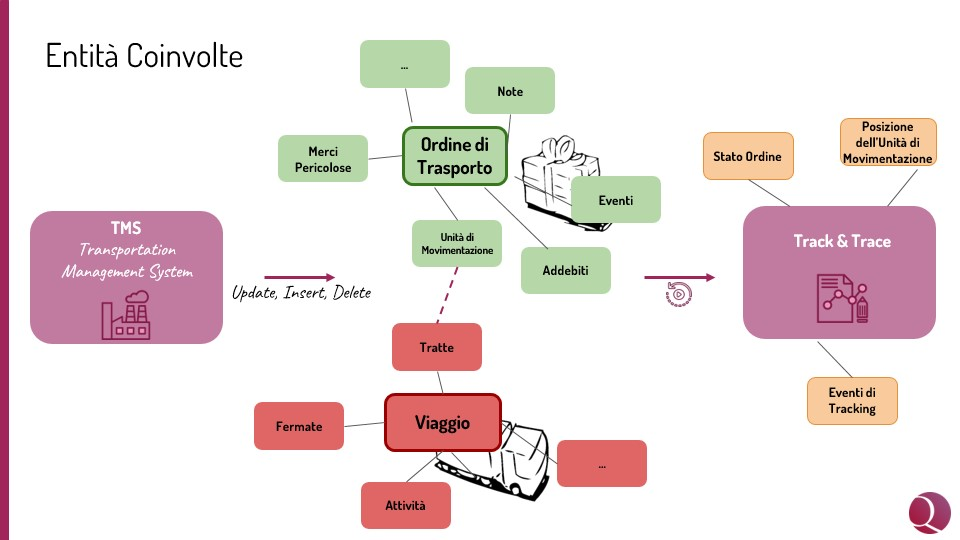
\includegraphics[width=\textwidth]{images/architecture/entita_coinvolte.jpg}
    \caption{Entità coinvolte}
    \label{fig:architecture_entities_img}
\end{figure}

La sorgente dei dati è il \textit{Transport Management System (TMS)} un software esterno che effettua modifiche a diverse entità.
Con il termine \textbf{Entità} si intende qualsiasi caratteristica che definisce un oggetto o situazione reale, ad esempio un \textit{viaggio} potrebbe avere le seguenti entità:
\textit{origine,destinazione, durata, etc ...}\\
Nel sistema le entità sono raggruppabili in diversi domini, i cui 3 principali sono:
\begin{itemize}
    \item Ritiro
    \item Ordine di trasporto (Spedizione)
    \item Viaggio
\end{itemize}
In figura \ref{fig:architecture_entities_img} sono presentati due domini d'esempio, \textit{Viaggio} e \textit{Ordine di Trasporto}.
I vari domini non sono isolati l'uno dall'alto, bensì la modifica di una entità potrebbe implicare la modifica di un'altra entità.
In figura \ref{fig:architecture_entities_img} ad esempio modificando una \textit{unità di movimentazione} verrebbe conseguentemente modificata una \textit{tratta}.
\\
\\
Lo scopo del sistema di \textbf{T\&T} è proprio quello di tenere traccia di tutti i cambiamenti subiti dalle varie entità (effettuati dal \textbf{TMS}).
Ciò avviene tramite \texttt{Debezium} (sezione \ref{sec:debezium_overview}) che monitora i database del \textbf{TMS} generando eventi di dominio, che verranno poi processati da altri microservizi.
%nel video quello che io chiamo entità vengono chiamati "root aggregate", anzi ancora diverso. sono tutte entità, ma le entità "viaggio" o "ordine trasporto" sono dei Root Aggregate, cioè degli oggetti che si portano dietro molte altre informazioni.
Il \textbf{T\&T} si occupa anche di fornire ai clienti informazioni sullo stato e sulla storia di diversi oggetti, composti dalle entità.
Ad esempio potrebbe essere fornito l'oggetto \textit{Carico} che descrive lo spostamento di un mezzo e tutte le consegne effettuate,
quindi costituito da \textit{Tratta e Fermate} ma anche dalle informazioni riguardo alle merci che trasporta, cioè \textit{Note,Unità di movimentazione, etc ...}

\section{Track and Trace legacy}
\label{sec:T&T_old}
Sistema basato su Batch, a regolari intervalli di tempo il sistema va a vedere il nuovo stato delle entità ed aggiorna un suo database interno di oggetti composti.
\todo{chiedere più info}

\section{Progetto Velocity}
\label{sec:T&T_new}
Sistema \textit{Event Driven} basato su \texttt{Kafka Streams}. (sezione \ref{subsubsec:kafka_stream})
Quando una entità cambia stato la modifica viene registrata su un \texttt{Kafka Topic} e, successivamente, gli eventi sui Topic vengono analizzati o filtrati tramite \texttt{Kafka Stream}.
Possiamo distinguere 3 tipologie di \texttt{Kafka Topic}:
\begin{figure}[H]
    \centering
    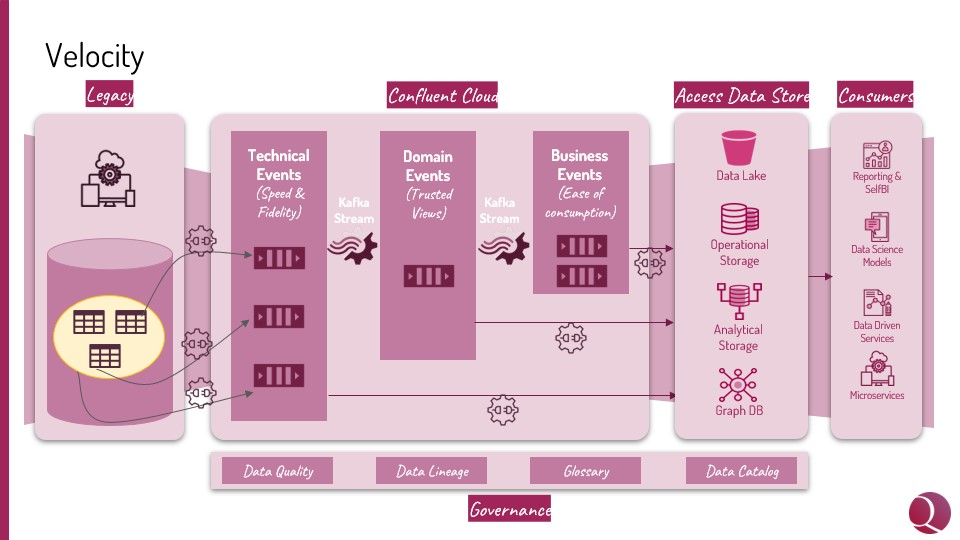
\includegraphics[scale=0.5]{images/architecture/confluent_velocity.jpg}
    \caption{Tipologie di Kafka Topics}
    \label{fig:kafka_topics.img}
\end{figure}
\begin{itemize}
    \item \textbf{Technical Events}: Contengono gli eventi generati dal \textbf{TMS}, sono eventi molto simili a dei log di un database
    (essendo generati tramite \texttt{Debezium} sono sostanzialmente una collezione di operazioni SQL) e spesso sono ridondanti, è
    infatti comune che il sistema effettui operazioni poco efficienti.
    Ad esempio qualora io avessi un ordine con una nota e la volessi modificare il TMS potrebbe svolgere la richiesta segnalando una operazione di \texttt{DELETE} ed una di \texttt{INSERT} piuttosto che effettuare una semplice \texttt{UPDATE}.\\
    É presente un \texttt{Topic} di tipo \textit{Technical Events} per ogni tabella del database originale (quindi un topic ogni dominio).
    \item \textbf{Domain Events}: Questi Topic contengono gli eventi filtrati dai \textit{Technical Events} tramite i \texttt{Kafka Streams}, non sono più simili a dei log di un DB (già solo la loro struttura è JSON, non SQL) e rappresentano come è fatto un oggetto (ordine di trasporto, viaggio, ...). 
    Tutti i potenziali eventi ridondanti sono stati filtrati dallo \textit{Stream}, non vi è più quindi il problema degli eventi ridondanti.
    \item \textbf{Business Events}: \texttt{Topic} opzionali, contengono degli eventi strutturati come i consumatori si aspettano (Ease of consumption). Sono pensati per fornire una vista specifica per un particolare consumer.
\end{itemize}

\subsection{Problema della consistenza}
\todo{farlo?}

\subsection{Componenti}
\label{subsec:components}

\subsubsection{Kafka Streams}
\label{subsubsec:kafka_stream}
\texttt{Kafka Streams} è una API per processare eventi su un \texttt{Topic Kafka} (filtrare, trasformare, aggregare, ...), questo tema viene approfondito nella sezione \ref{subsec:kafka_streams}\\
\\
Gli \texttt{Stream} che collegano i \texttt{Topic} di tipo \textit{Domain Events} a quelli di tipo \textit{Domain Business Event} sono molto dipendenti dalle necessità del consumatore che poi li leggerà quindi non seguono una struttura fissa.
Invece gli \texttt{Stream} che leggono dai \textit{Technical Events Topic} seguono una struttura precisa e svolgono operazioni suddivisibili in 3 fasi:
\begin{enumerate}
    \item \textbf{Fase di Casting}.\\
    In questa fase avviene la ricostruzione dell'evento basandosi sui log generati da \texttt{Debezium} che sta osservando il \textbf{TMS}.\\
    \texttt{Debezium} si occupa di rilevare ogni cambiamento e pubblica l'evento su diversi topic kafka, uno per tabella (quindi uno per ogni dominio). 
    \item \textbf{Fase di Filtro}\\
    Successivamente gli eventi ridondanti devono essere eliminati. Tutti gli eventi relativi ad una transazione vengono accorpati e viene generato un unico evento risultante, che non riporta gli eventi intermedi. 
    \item \textbf{Fase di Mapping}\\
    Il nuovo evento viene quindi trasformato in un \textit{Domain Event} ed inserito sul relativo Topic.
\end{enumerate}

\subsubsection{MicroBatch}
\label{subsubsec:micro_batch}
Questo microservizio si occupa di "ricostruire" una entità a partire da tutti gli eventi che la riguardano. 
Non legge direttamente dal Topic \textit{Domain Events} quindi non è un \textit{consumer Kafka} bensì legge gli eventi di dominio da elaborare da un database SQL chiamato \texttt{Fast Storage}
che viene continuamente aggiornato da un connettore JDBC.
Gli eventi che riceve in input sono quindi dei \textit{Domain Events}, già filtrati dai relativi \texttt{Kakfa Stream}.\\
Dopo la "ricostruzione" l'oggetto viene riscritto nel Fast Storage, eliminando da esso gli eventi che lo riguardavano e che non sono più necessari.
Il microservizio \texttt{MicroBatch} è scritto usando \textit{Spring Batch} e lo scheduler su cui si appoggia per eseguire i Job è \textit{Quartz}.\\\\
Il primo passo, svolto ogni 5 secondi, è un partizionamento. Una classe \texttt{Spring Batch} chiamata \textit{Partitioner} divide gli eventi di dominio in \textit{chunks}, in modo da poterli processare in parallelo.
Il numero di \textit{chunks} è liberamente configurabile, ma il partizionatore è scritto in modo da raggruppare gli eventi con la stessa chiave di dominio (cioè relativi alla stessa Transazione) nella stessa partizione.
Questo non garantisce però che all'interno di un \textit{chunk} ci siano solo eventi con la stessa chiave di dominio.
A questo punto vengono eseguiti i vari \textit{Jobs}, uno per ogni \textit{chunk}, la cui esecuzione si può suddividere in 3 passi.
\begin{enumerate}
    \item \textbf{Reading}: Durante la fase di \textit{Reading} vengono recuperati dal Fast Storage tutti gli Eventi di Dominio che sono stati assegnati dal Partizionatore a quello specifico \textit{chunk}.
    \item \textbf{Processing}: Fase in cui si trasformano gli Eventi di Dominio recuperati durante la fase di \textit{Reading} in una serie di record pronti alla scrittura, ovvero in una serie di oggetti di tipo \texttt{Entity}.
    Le \textit{Entità} andranno quindi a comporre degli oggetti di vario tipo, infatti \texttt{MicroBatch} non si occupa di tenere aggiornata una sola tabella, bensì diverse tabelle sullo stesso database. \todo{quando avro accesso al DB potrò inserire questi esempi}
    Quindi partendo dagli stessi Eventi di Dominio verranno generati diversi record (diverse \texttt{Entity}) che verranno scritti su diverse tabelle.
    \item \textbf{Writing}:Fase finale di scrittura sul Fast Storage. É una scrittura transazionale, quindi deve rispettare le proprietà \texttt{ACID}, requisito di cui si occupa il \textit{Job}.
    Inoltre il \textit{Job} si occupa di verificare per ciascuna tabella se i dati che ha generato devono essere inseriti o solamente aggiornati.
\end{enumerate}

\subsubsection{Event Engine}
\label{subsubsec:event_engine}
Similmente a \texttt{Micro Batch} (sezione \ref{subsubsec:micro_batch}) l'\textit{Event Engine} si occupa di "costruire" degli oggetti di business partendo dal \textit{Fast Storage}, questi oggetti sono pensati per la \textit{ease of consumption} di eventuali client.\\
In altre parole si occupa di osservare i cambiamenti di stato dei diversi eventi di dominio (segnalati dall \textbf{SGA} che monitora il \textbf{TMS}) e generare una serie di eventi di business associati (es: 
“spedizione partita”, “ritiro fallito”, “arrivo stimato”, …)\\\\
Rispetto al caso \texttt{Micro Batch} (\ref{subsubsec:micro_batch})la fase di \textit{Reading} ritorna solo un record per ogni chiave di dominio,
quindi ad ogni \textit{chunk} corrisponde una e solo una chiave di dominio.
Invece le tre altre due fasi (\textit{Processing e Writing}) sono sostanzialmente identiche, con la differenza che la fase di Processing non va a generare un oggetto, bensì calcola una serie di metriche come "orario di partenza", "Tragitto", "Stato dell'ordine", etc ....
\chapter{Tecnologie utilizzate}
\label{ch:Tecnologies}

\section{Apache Kafka}
\label{ch:kafka_overview}
%https://kafka.apache.org/intro
\textit{Apache Kafka is an open-source distributed event streaming platform.}\cite{kafkawebsite}\\\\
\texttt{Apache Kafka} è una piattaforma open-source per l'archiviazione e l'analisi di flussi di dati.
Si basa sul concetto di \textit{Flusso di eventi}, cioè la pratica di catturare dati in real-time da diverse fonti (databases, sensori, software, ...) sotto forma di \textbf{Eventi}.\\
Un \textbf{Evento} è un record all'interno del sistema di qualcosa che si è verificato (il rilevamento di un sensore, un click , una transazione monetaria, etc ...). In Kafka un evento è costituito da una \textit{key}, un valore, un \textit{timestamp} ed eventualmente altri metadati. Un esempio di evento potrebbe essere il seguente:
\begin{itemize}
    \item \textbf{Key}: Alice
    \item \textbf{Value}: "Pagamento di 200€ a Bob"
    \item \textbf{timestamp}: 1706607035
\end{itemize}
\texttt{Kafka} può eseguire 4 operazioni su un \textbf{Evento}:
\begin{itemize}
    \item \textbf{Scrittura}: L'evento può essere generato da un \textit{Producer}(\ref{subsec:kakfa_clients}) che lo pubblica all'interno di un \textit{Topic}.
    \item \textbf{Lettura}: L'evento può essere letto da un \textit{Consumer}(\ref{subsec:kakfa_clients}) che è iscritto ad un \textit{Topic} e ne riceve gli aggiornamenti.
    \item \textbf{Archiviazione} o \textbf{Storage}: Un evento può essere salvato su un \textit{Topic} in maniera sicura e duratura. Differentemente da un \texttt{Message Broker}, che offre le stesse funzionalità di lettura e scrittura, i record all'interno di un \textit{Topic} sono permanenti, questo argomento è maggiormente approfondito nella sezione \textit{Topic}(\ref{subsec:kafka_topics})
    \item \textbf{Elaborazione}: Gli \textbf{Eventi} possono essere elaborati, sia in gruppo che singolarmente, questa elaborazione può essere effettuata tramite i cosiddetti \texttt{Kafka Streams}(\ref{subsec:kafka_streams})
\end{itemize}
In ultimo \texttt{Kafka} è un sistema distribuito, è quindi possibile avere più istanze, dette \texttt{Kafka Brokers}, che collaborano in un \texttt{Kafka Cluster}. Grazie a questa caratteristica si possono implementare meccanismi di parallelizzazione, high-availability e ridondanza.
In particolare su ogni \texttt{Broker} sono salvati uno o più \textit{Topic} ed i differenti endpoints (siano essi \textit{Consumers,Producers,Streams o Connectors}) vi dialogano per leggere o scrivere sui \textit{Topic}.
Un \texttt{Cluster} di esempio è mostrato in figura \ref{fig:kafka_cluster}
\begin{figure}[htbp]
    \centering
    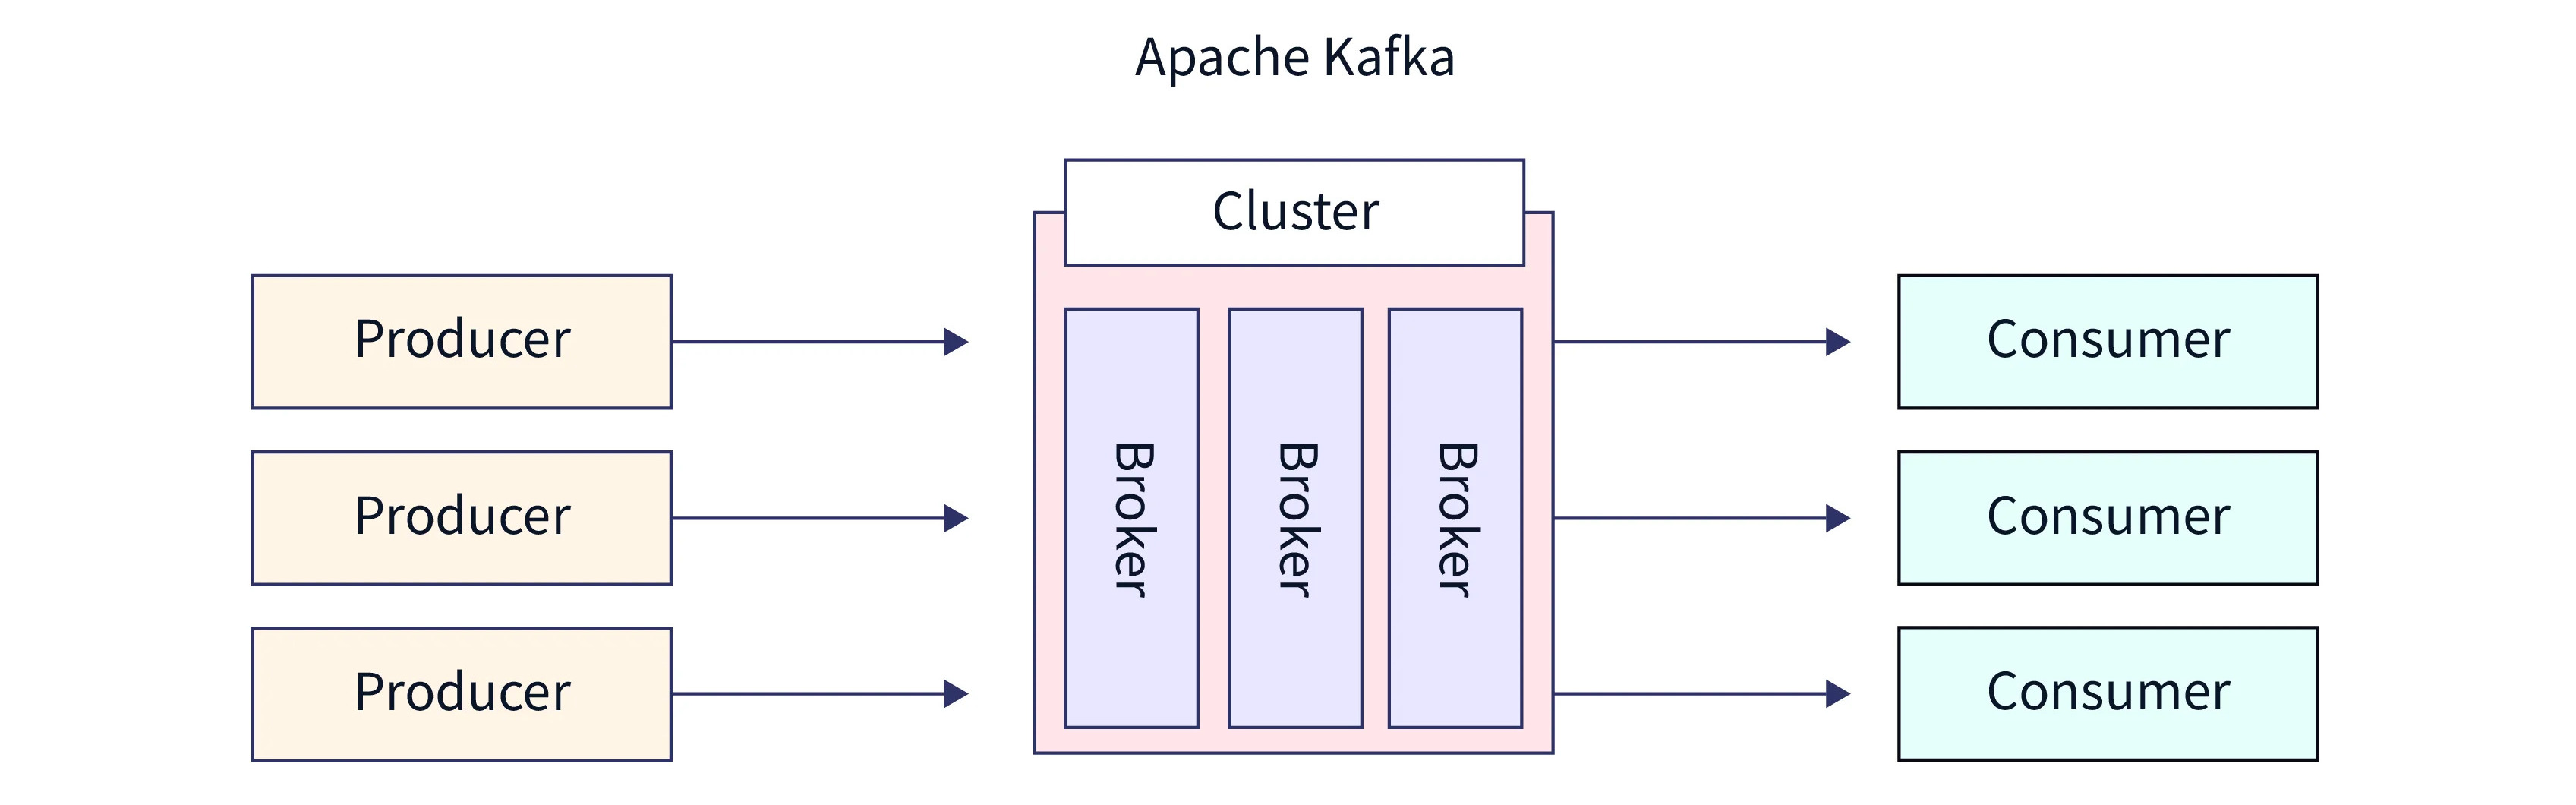
\includegraphics[width=\textwidth]{images/kafka/cluster.jpg}
    \caption{Kafka Cluster}
    \label{fig:kafka_cluster}
\end{figure}
% dovrei citare la fonte della figura https://www.scaler.com/topics/kafka-cluster/

\subsection{Topic}
\label{subsec:kafka_topics}

Un \textit{Kafka Topic} è un database ad eventi, al posto di pensare in termini di oggetti, si pensa in termini di eventi.
Diversi microservizi possono consumare o pubblicare sullo stesso \textit{Topic}, similmente ad un \texttt{Message Broker} infatti i \textit{Topic} sono \textit{multi-producer} e \textit{multi-subscribers}.
A differenza di un \texttt{Message Broker} però un \textit{Topic} può mantenere dei record in maniera sicura per una durata di tempo indefinita, come se fosse un database.Gli \textbf{Eventi} infatti non sono eliminato dopo esser stati letti da un \textit{Consumer}. Il tempo di mantenimento di un record può essere configurato in modo da stabilire un equilibrio tra quantità di dati salvati e efficienza delle elaborazioni dato che ad un numero maggiore di record corrisponde un tempo di elaborazione maggiore.\\\\
I \textit{Topic} sono partizionati, per permettere high-availability, fault-tollerance e soprattutto consentire la lettura/scrittura in parallelo.
Infatti ogni \textit{Topic} è distribuito tra vari \textit{buckets}, che si trovano nei \texttt{Kafka Brokers}.
Eventi aventi la stessa \textit{Key} sono scritti nella stessa partizione e \textit{Kafka} garantisce che qualsiasi \textit{Consumer} iscritto a tale partizione leggerà gli eventi nello stesso ordine in cui sono stati scritti.
Come citato prima il partizionamento permette anche la scrittura in parallelo, infatti se la partizione su cui due \textit{Producer} scrivono è differente e possibile effettuare l'operazione senza doversi preoccupare dei problemi generati dalla scrittura concorrente, anche se il \textit{Topic} è il medesimo.
Un esempio di partizionamento è mostrato in figura \ref{fig:kafka_topic}
\begin{figure}[htbp]
    \centering
    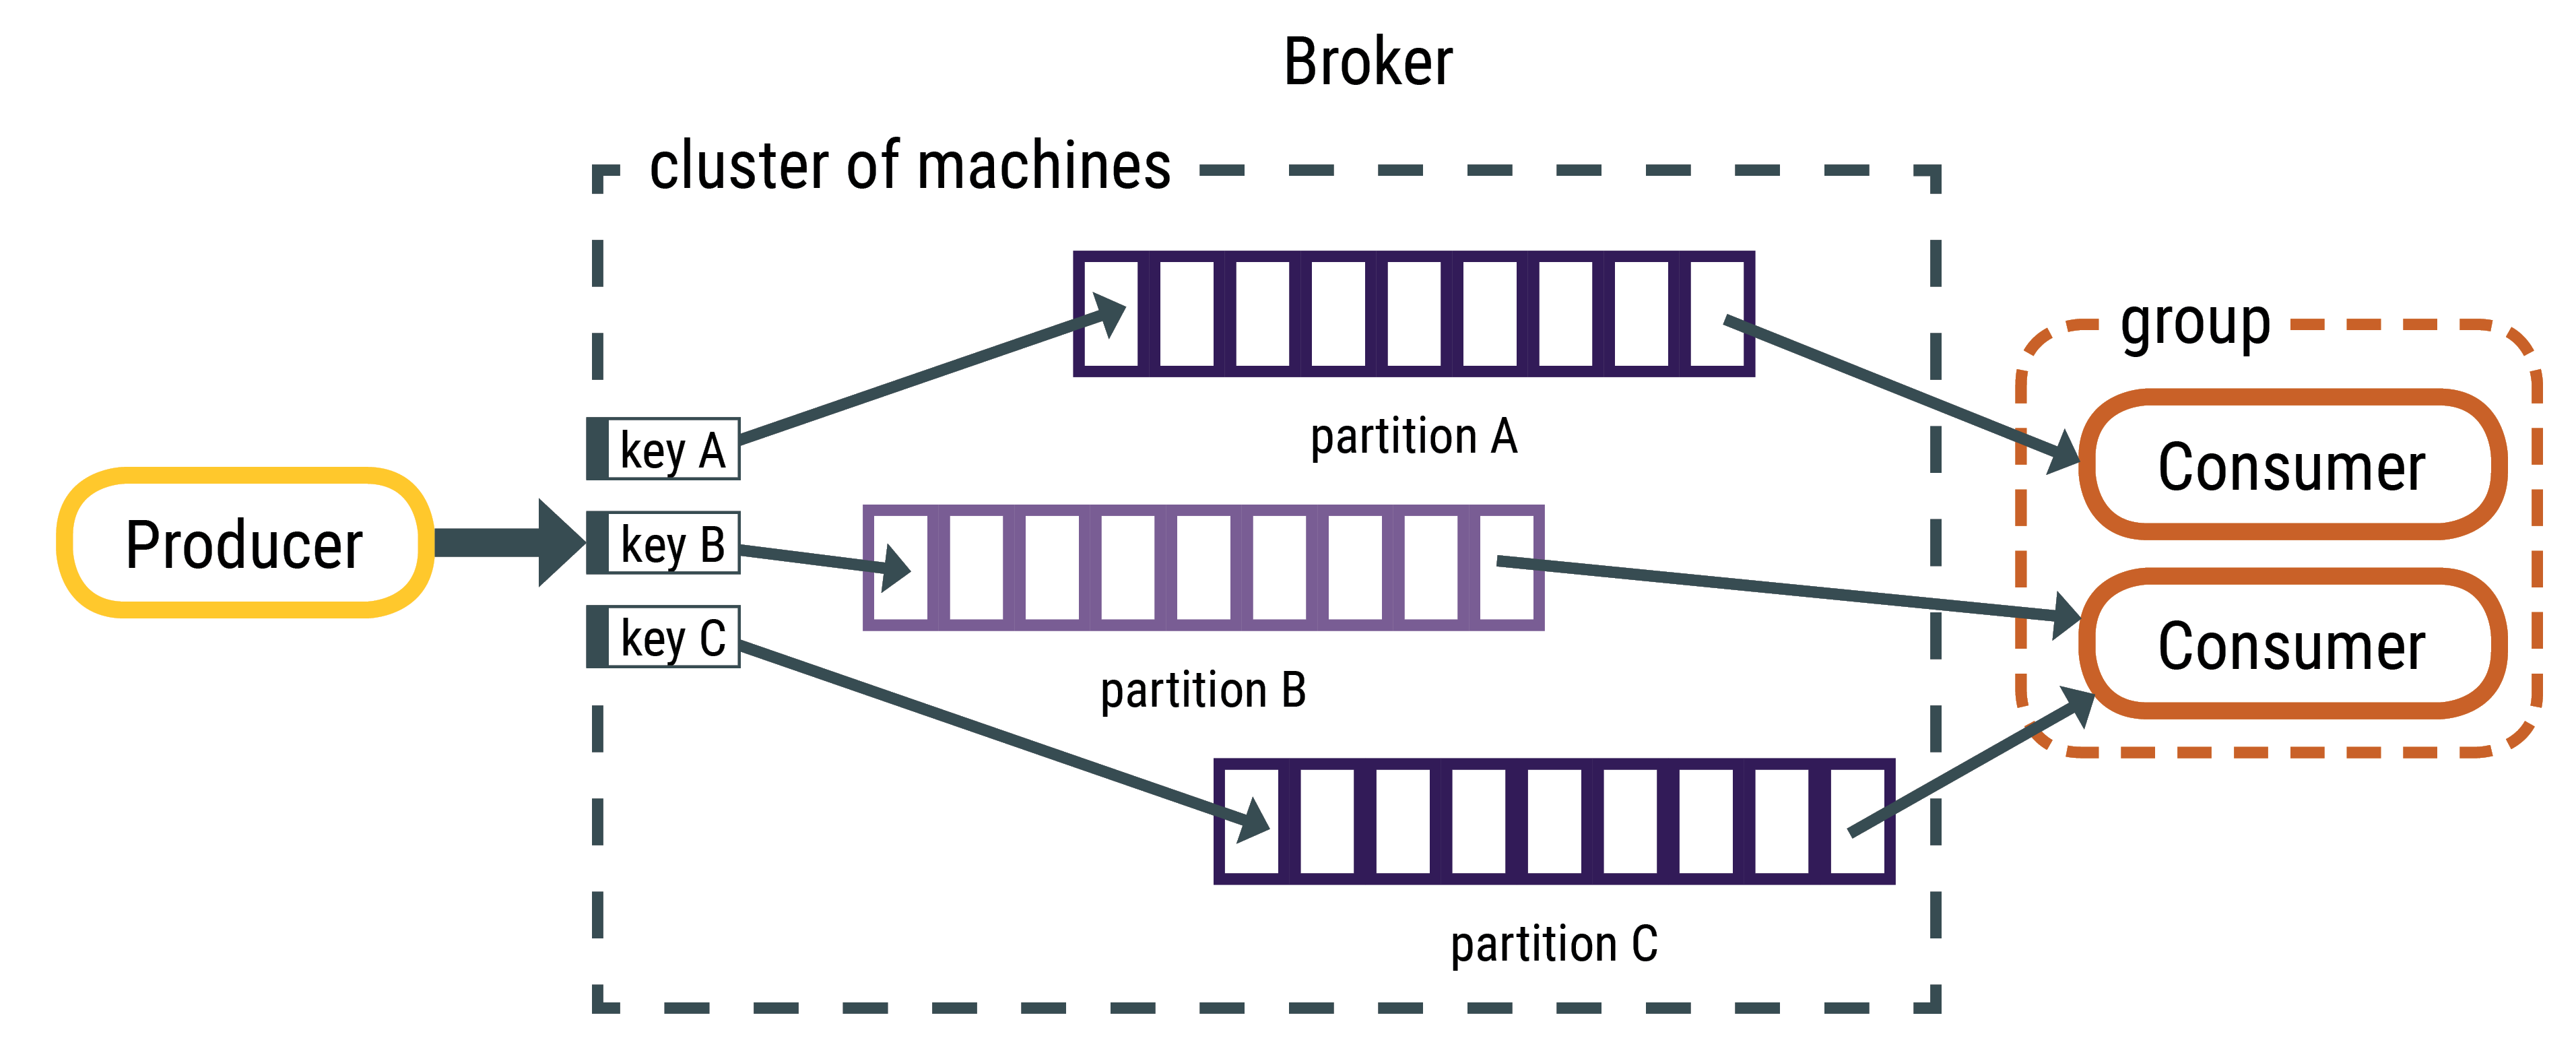
\includegraphics[width=0.9\textwidth]{images/kafka/topic.png}
    \caption{Partizionamento Kafka Topic}
    \label{fig:kafka_topic}
\end{figure}
%https://docs.datastax.com/en/kafka/doc/kafka/kafkaHowMessages.html

\subsection{Clients}
\label{subsec:kakfa_clients}
I \texttt{Consumers} ed i \texttt{Producers}, insieme ai \textit{Topics}, sono gli elementi alla base del funzionamento di \textit{Kafka}.
Il \textit{Cluster Kafka} composto dai vari \textit{Brokers} svolge il ruolo di \textbf{Server}, mentre i \texttt{Consumers} ed i \texttt{Producers} fungono da \textbf{Clients},
collegandosi al cluster e interagendo con i dati presenti sui \textit{Topics}.
I \textit{Clients} sono i componenti che si occupano di implementare la logica di business e sono quindi scritti dallo sviluppatore che sfruttera le due API messe a disposizione da Kakfa,
\textit{Consumer API} e \textit{Producer API}

\subsection{Streams}
\label{subsec:kafka_streams}
\texttt{Kafka Streams} è una API per processare eventi su un \texttt{Topic Kafka} (filtrare, trasformare, aggregare, ...).
Ad esempio se volessi sapere quanti ordini di trasporto sono stati spediti oggi, potrei fare un filtro per data e poi un count, quello il \texttt{Kafka Stream} fornirà in output sarà un altro flusso di dati filtrato, che potrò salvare su un nuovo \texttt{Topic} o in un database.\\
Nascono con l'intenzione di "astrarre" tutte le operazioni di basso livello quali la lettura o la scrittura su un \textit{Topic}, permettendo allo sviluppatore di preoccuparsi solamente di come i dati devono essere modificati, senza dover scrivere codice per ottenerli o ripublicarli.
In pratica qualsiasi operazione implementabile tramite \texttt{Kafka Streams} sarebbe allo stesso modo implementabile da un microservizio che legge da un \textit{Topic}, elabora i dati e li riscrive su un \textit{Topic}(lo stesso o un altro), ma grazie agli \texttt{Streams} si possono delegare le operazioni di collegamento con il \texttt{Kakfka Cluster} e concentrarsi solamente sull'elaborazione dei dati.
L'utilizzo dei \texttt{Kafka Streams} ha i seguenti vantaggi:
\begin{itemize}
    \item Efficienza: Il tipo di computazione è per-record, cioè ogni dato pubblicato sul \textit{Topic} a cui lo \texttt{Stream} è collegato viene subito processato. Non c'è bisogno di effettuare "batching", cioè richiedere i dati ad intervalli di tempo regolari ed elaborare solo i dati giunti in tale intervallo. Il sistema può lavorare quasi in tempo reale.  
    \item Scalabilità: Gli \texttt{Stream} sono scalabili e fault-tollerant. Essendo \textit{Kafka} pensato per essere un sistema distribuito anche gli \texttt{Streams} sono pensati per essere scalati e distribuiti, se si creano diverse istanze dello stesso \texttt{Stream} queste collaboreranno automaticamente suddividendosi il carico computazionale.
    \item Riuso del codice: si utilizza una chiamata all API al posto di riscrivere lo stesso codice per differenti microservizi.
\end{itemize}

\subsection{Connector}
\label{subsec:kafka_connectors}
I \texttt{Connectors} sono particolari tipi di \texttt{Consumers/Producers}, il cui scopo è mettere in comunicazione \textit{Kafka} con altri sistemi.
I \texttt{Connectors} producono flussi di eventi partendo da dati ricevuti da un altro sistema (\textit{Source Connector}), oppure consumano da un topic e inviano i dati letti ad una applicazione esterna(\textit{Sink Connector}).
Per esempio un \texttt{Connector} ad un database relazionale potrebbe catturare tutte le operazioni effettuate su una tabella e generare un flusso di eventi in cui ogni evento corrisponde ad un cambiamento.
Similmente ai \textit{Kafka Streams} \ref{subsec:kafka_streams} i principali vantaggi di utilizzare un \texttt{Connector} piuttosto che scrivere da se il codice per svolgere lo stesso compito sono
\textbf{efficienza},\textbf{scalabilità} e \textbf{riuso del codice}.
Inoltre sono presenti diversi repository online dove trovare \texttt{Connector} già pronti, sviluppati dalla community o dagli sviluppatori delle applicazioni esterne (sqlserver, JDBC, Amazon S3),
uno dei più diffusi è il \texttt{confluent-hub} https://www.confluent.io/product/connectors/ \todo{questo deve diventare un link o essere spostato in bibliografia}

\section{Debezium}
\label{sec:debezium_overview}
\textit{Debezium is an open source distributed platform for change data capture. Start it up, point it at your databases, and your apps can start responding to all of the inserts, updates, and deletes that other apps commit to your databases.}\cite*{debeziumwebsite}\\\\
\texttt{Debezium} è una piattaforma distribuita open source per la cattura dei dati di modifica, permette di catturare le operazioni di modifica effettuate su un database (\textit{insert, update e delete}) e di trasformarle in eventi.
Nativamente tutti i più comuni database sono supportati, tra cui \textit{MySQL, PostgreSQL, MongoDB, SQL Server, Oracle, ...}.\\\\
\texttt{Debezium} è costruito sulla base di \textit{Apache Kafka}, di conseguenza è facilmente integrabile con esso.
Ci sono infatti due modi per utilizzare questa piattaforma: come un sistema distriubuito a se stante oppure tramite un \texttt{Kafka Connector}(\ref{subsec:kafka_connectors}).
Il primo modo presenta tutti i vantaggi di un sistema distribuito, come la scalabilità e la fault-tollerance, ma ha un costo in termini di risorse, di configurazione e di gestione.
È inoltre possibile consumare gli eventi prodotti tramite un qualsiasi sistema esterno, senza dover necessariamente utilizzare \textit{Kafka}.
Se invece si ha già una infrastruttura già basata su \textit{Kafka} è molto più conveniente utilizzare \texttt{Debezium} come \texttt{Connector}, con un considerevole risparmio di risorse e di tempo.  

\section{Apache Flink}
\label{sec:flink_overview}
\textit{Apache Flink is a framework and distributed processing engine for stateful computations over unbounded and bounded data streams. Flink has been designed to run in all common cluster environments, perform computations at in-memory speed and at any scale.}\cite*{flinkwebsite}\\\\

\textit{Apache Flink} è sia un framework che un motore di elaborazione distribuito per la computazione di flussi di dati, \textit{bounded} e \textit{unbounded}.
Può essere utilizzato per elaborare dati in tempo reale, ma anche per elaborare grandi quantità di dati in batch.
Fornisce sia una API per la creazione di applicazioni di elaborazione di dati, sia un \textit{runtime} environment distribuito per eseguirle,
per questo motivo si può considerare sia un \textit{framework} che un \textit{motore di esecuzione}.
Come anticipiato i tipi di dato trattato sono sempre \texttt{streams} che possono essere:
\begin{itemize}
    \item \textbf{Unbounded}: un flusso di dati che non ha un inizio o una fine, come ad esempio un flusso di eventi generati da un sensore.
    \item \textbf{Bounded}: un flusso di dati con un inizio e una fine, come ad esempio un file o una tabella di un database.
\end{itemize}
Sui flussi \textit{Bounded} possono essere eseguite tutte le operazioni eseguibili sui flussi \textit{Unbounded}, ma non viceversa.
Per fare ciò bisogna ricorrere a delle operazioni di \textit{windowing}, cioè dividere il flusso in finestre (temporali o di conteggio 
\footnote{Per \textit{finestra di conteggio} si intende una finestra che contiene un numero fisso di elementi, ad esempio una finestra di 100 elementi.
In inglese si parla di \textit{count window}.}
) e poi eseguire le operazioni su queste finestre.

\subsection{Statefull stream processing}
\label{subsec:flink_statefull_processing}
\textit{Flink} può svolgere operazioni che richiedono il mantenimento di uno stato, cioè un insieme di informazioni riguardanti gli eventi passati.
Semplici esempi di elaborazioni che richiedono uno stato sono: la ricerca di un pattern, il calcolo di una media (mobile se si parl di \textit{Stream Unbounded}), il calcolo di una somma, etc \dots
\textit{Flink} sfrutta il lo stato anche per garantire la \textit{fault-tollerance}, cioè la capacità di ripristinare il sistema in caso di guasto.\\\\
Il metodo più comune con cui una applicazione \textit{Flink} sfrutta lo \textit{Statefull processing} è tramite l'uso di \textit{Keyed Stream}.
Operando su un \texttt{Datastream} può essere effettuata una operazione di \texttt{keyBy} che permette di raggruppare gli eventi in base ad una chiave,
in modo che tutti gli eventi con la stessa chiave appartengano alla stessa partizione logica.
Si ottiene quindi un \texttt{KeyedStream} su cui è possibile eseguire operazioni di \textit{statefull processing}, 
il seguente codice di esempio mostra come calcolare la somma di un \texttt{KeyedStream} di ogetti composti da una chiave (\textit{f0}) e un valore(\textit{f1}):

\begin{code}
    \inputminted{java}{listings/keyed-stream.java}
    \caption{Esempio di operazione statefull su un KeyedStream}
    \label{lst:keyed_stream}
\end{code}


Oltre ad essere necessario per mantenere uno stato il partizionamento tramite chiave permette anche di parallelizzare le operazioni, 
dato che ci assicura non ci saranno conflitti tra le operazioni eseguite su partizioni diverse.
Nell'esempio precedente (listing \ref{lst:keyed_stream}) la somma potrebbe venire calcolata in parallelo per ogni chiave, dato che lo stato mantenuto dal sistema
,che corrispone semplicemente alla variabile \texttt{accumulator}, non viene mai acceduto durante la computazione di un dato avente un'altra chiave.
posto naturalmente che si abbia a disposizione sufficienti risorse computazionali.
Il discorso di come \textit{Flink} gestisca le risorse è approfondito nella sezione \ref{subsubsec:flink_Task_slots}.

\todo{parlare del checkpointing?}

\subsection{Windowing}
\label{subsec:flink_windowing}

\subsection{Flink Cluster}
\label{subsec:flink_cluster}
Un \textit{Flink Cluster} è penasto per essere eseguito in un ambiente distribuito, come ad esempio un \textit{Hadoop YARN, docker} o \textit{Kubernetes},
ma non è limitato a ciò, può essere eseguito anche in un ambiente \textit{standalone} oppure si può sfruttare solo la API di Flink senza dover necessariamente eseguire un \textit{Cluster}.
\begin{figure}[htbp]
    \centering
    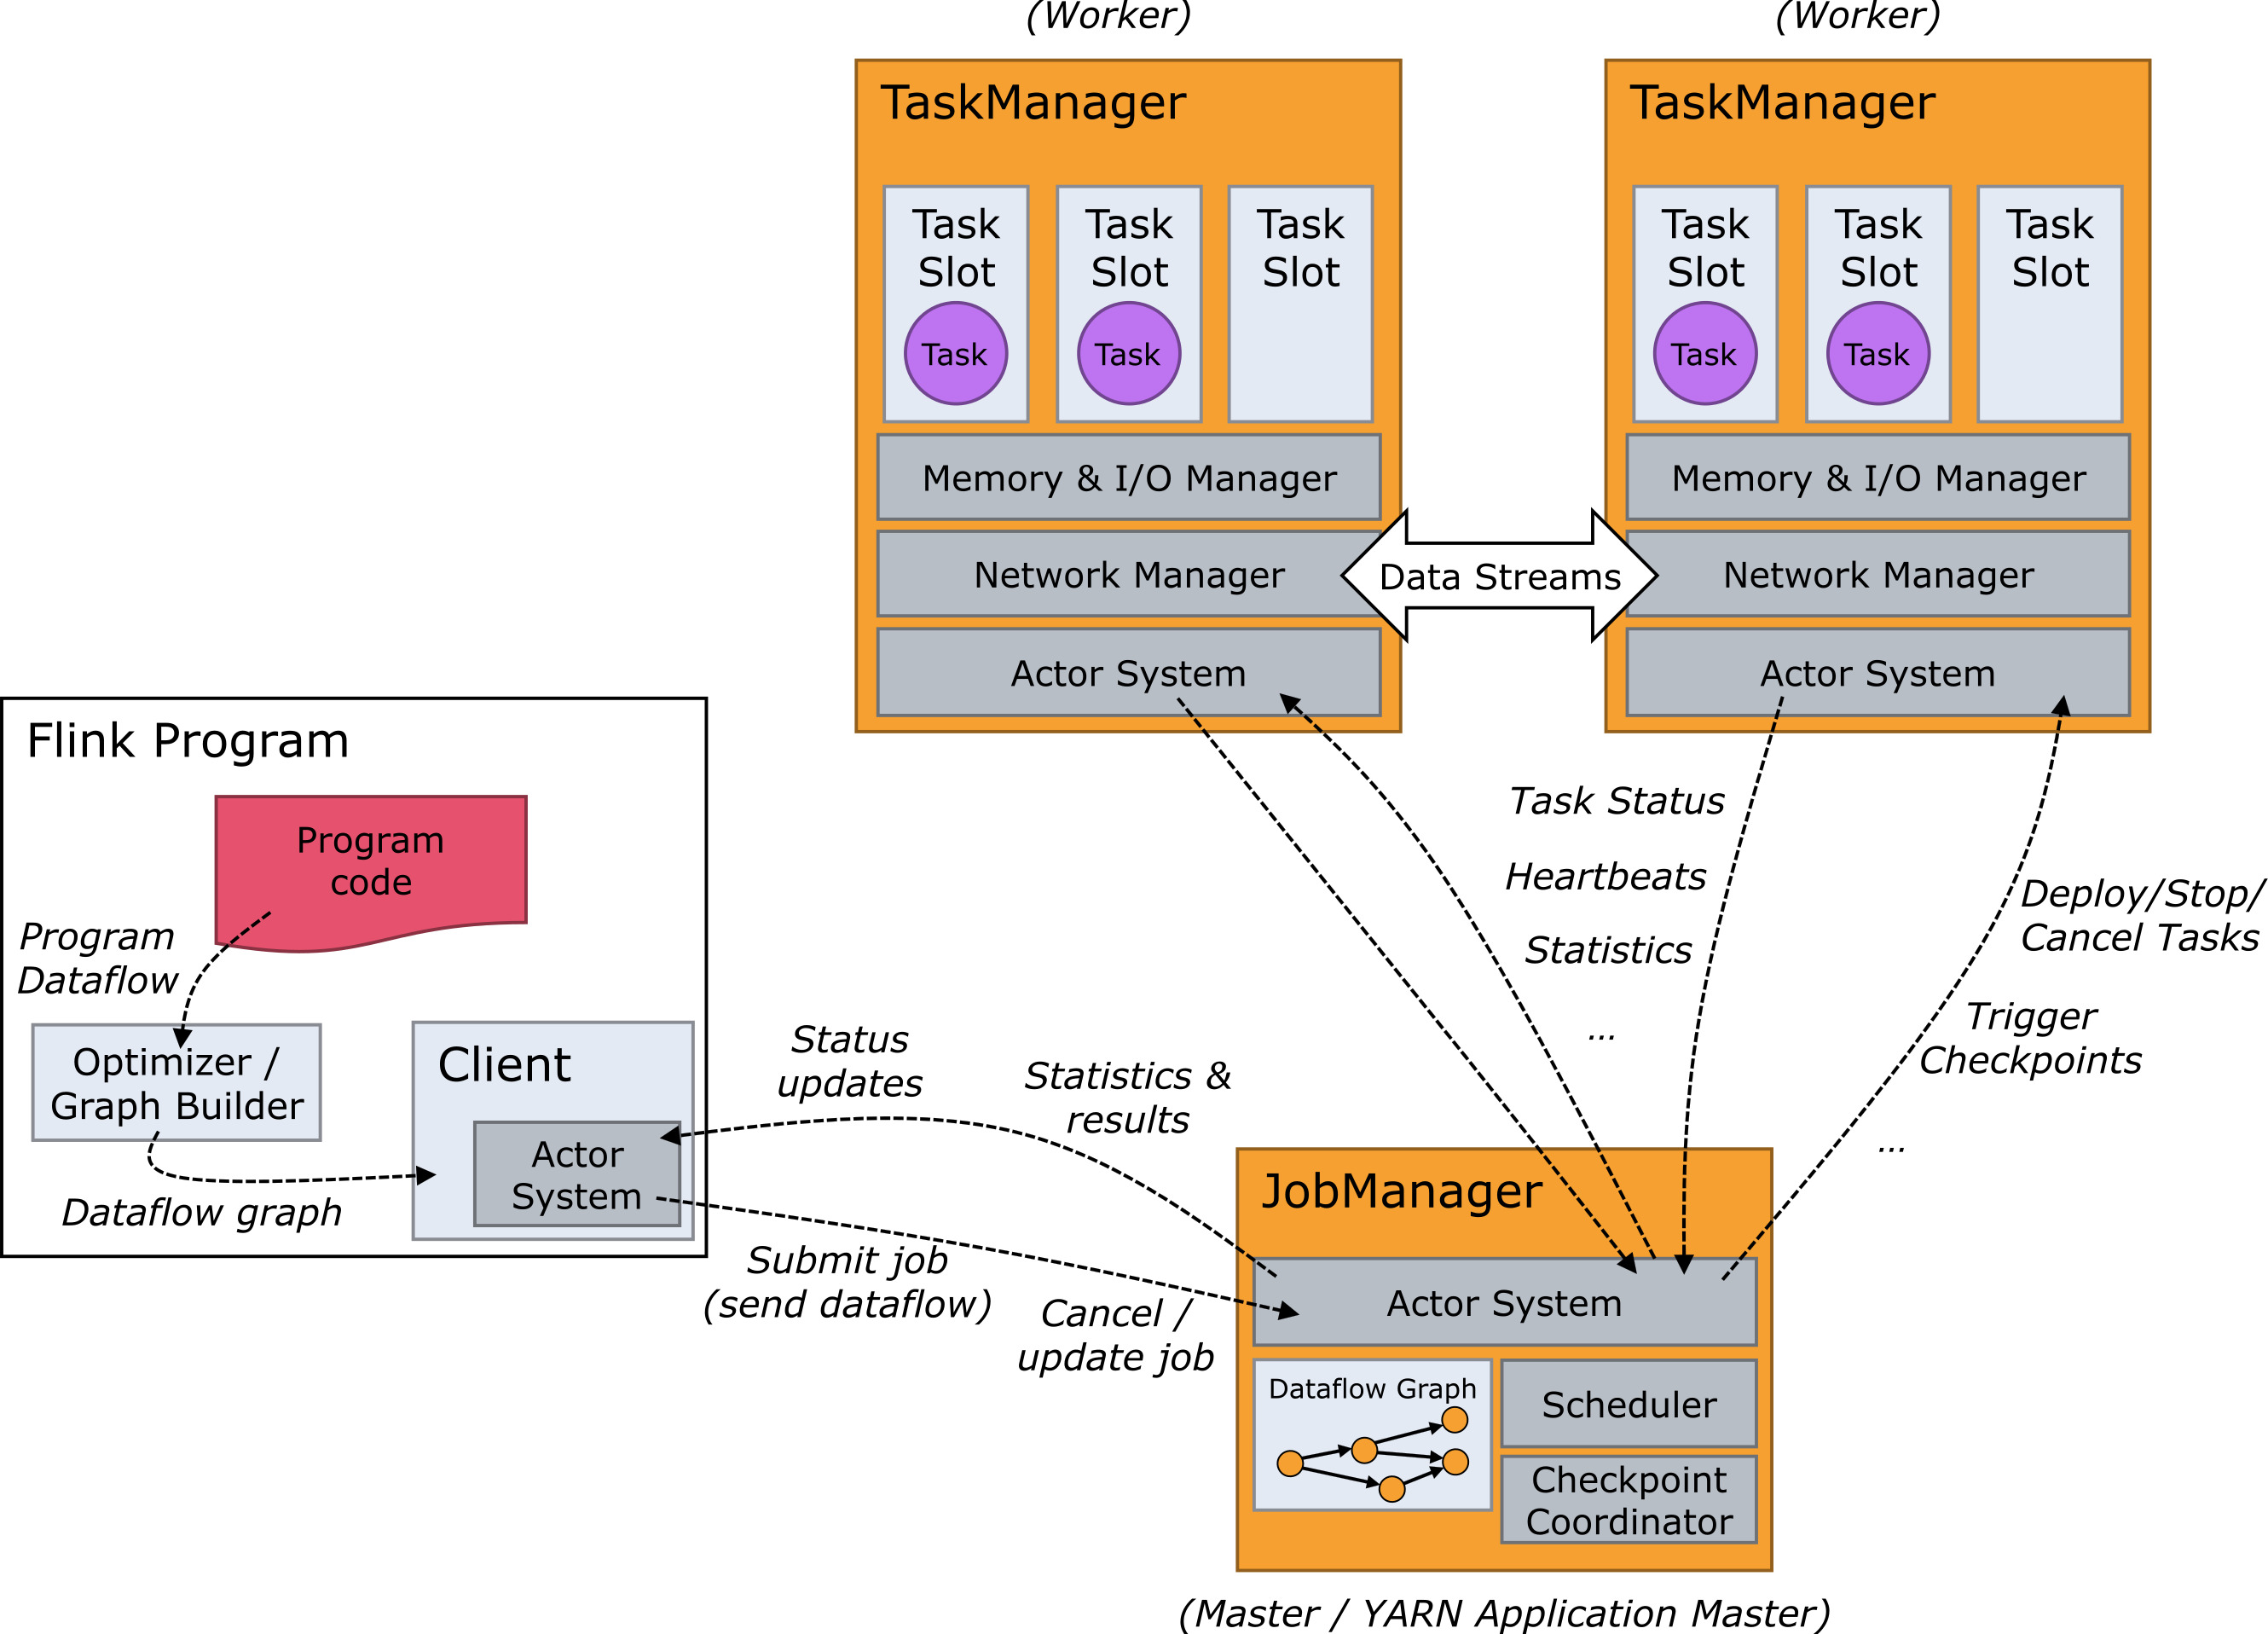
\includegraphics[width=\textwidth]{images/flink/cluster.jpg}
    \caption{Flink Cluster}
    \label{fig:flink_cluster}
\end{figure}
Il \textit{runtime environment} di Flink è composto da due tipi di processi: un JobManager e uno o più TaskManager.
\begin{itemize}
    \item \textbf{JobManager}: è il master del \textit{Cluster}, si occupa di coordinare il lavoro dei \textit{TaskManager} decidendo quando eseguire un Task,
    gestire gli errori in fase di esecuzione ed effettuare checkpointing 
    \footnote{Il meccanismo di checkpoint è una strategia di \textit{fault tolerance} basata sul mantenere degli snapshots di vari componenti del sistema
    per poterlo ripristinare in caso di guasto}.
    Le principali responsabilità del \textit{JobManager} sono due: la gestione delle risorse e la gestione dei job.
    \begin{enumerate}
        \item \textbf{Gestione delle risorse}: il \textit{JobManager} gestisce i \textbf{Task Slots}\ref{subsubsec:flink_Task_slots} dei \textit{TaskManager}, cioè le risorse computazionali.
        Se l'ambiente di esecuzione è distribuito (come ad esempio \textit{YARN} o \textit{Kubernetes}) il \textit{JobManager} avviare nuove istanze di \textit{TaskManager} in base alle necessità.
        \item \textbf{Gestione dei job}: il \textit{JobManager} si occupa di ricevere i job da eseguire, di distribuirli tra i \textit{TaskManager} e di monitorarne l'esecuzione.
        Inoltre fornisce una REST API ed una interfaccia web per monitorare lo stato del cluster e per ricevere nuovi jobs.
    \end{enumerate}
    C'è sempre almeno un \textit{JobManager}. Una configurazione \textit{Hig-Availability} potrebbe avere più \textit{JobManager}, di cui uno è sempre il leader e gli altri sono in standby.
    \item \textbf{TaskManager}: sono i worker del \textit{Cluster}, si occupano di eseguire i Task e di ricevere e inviare i dati.
    La più piccola unità di esecuzione in un TaskManager è un \textit{Task Slot} \ref{subsubsec:flink_Task_slots}.
    Il numero di slot di Task in un TaskManager indica il numero di Task eseguibili in parallelo.
\end{itemize}

\subsubsection{Task Slots}
\label{subsubsec:flink_Task_slots}
Per comprendere il concetto di \textit{Task Slot} è necessario comprendere come viene gestito il\textit{parallelismo} in \texttt{Flink}.    
Un programma scritto tramite l'API di \texttt{Flink} non viene eseguito sequenzialmente, ma viene diviso in sottoprocessi che possono essere eseguiti in parallelo.
Ad esempio un semplice programma che riceve dei dati, li filtra e li salva su un database potrebbe essere diviso in tre sottoprocessi: ricezione, filtro e scrittura.
Questi tre sottoprocessi sono chiamati \textit{Task} e possono essere, parzialmente, eseguiti in parallelo.
Inoltre, come anticipato nella sezione \ref{subsec:flink_statefull_processing}, una operazione di \texttt{KeyBy()} suddivide uno stream in partizioni di dati
indipedenti tra loro, quindi tutte le operazioni su questi dati possono essere eseguite in parallelo.
Potenzialmente potremmo eseguire la computazione di questi dati ognuna in un \textit{Task} differente, avendo così un \textit{Task}per ogni partizione,
cioè per ogni \textit{key} presente nello stream.
Qualora non si abbia a disposizione sufficienti risorse computazionali per dedicare ad ogni partizione un \textit{Task} il \texttt{Flink runtime environment} 
automaticamente aggregherà più partizioni in un cosiddetto \textbf{Key Group} che verrà trattato come una qualsiasi altra partizione.
\\\\
Ogni \texttt{TaskManage} è sostanzialmente un processo che esegue la JVM ed il codice, quindi può eseguire uno o più sottoprocessi in diversi \textit{threads}.
Ogni \texttt{Task Slot} rappresenta un sottoinsieme di risorse computazionali di un \texttt{TaskManager}, ad esempio un \texttt{TaskManager}
con 3 \texttt{Task Slot} dedicherà 1/3 delle sue risorse a ciascun \texttt{Task Slot}.
Più \texttt{Task Slot} si hanno a disposizione, più \texttt{Task} si possono eseguire in parallelo, ma anche meno risorse si avranno a disposizione per ciascun \texttt{Task}.
Inoltre se due \texttt{Task} operano sugli stessi dati è possibile effettuare \textit{slot sharing}, cioè permettere a due \texttt{Task} di condividere un \texttt{Task Slot}, limitando il parallelismo ma riducendo il consumo di memoria.
Come si può vedere nell'immagine \ref{fig:flink_slots} dove i \texttt{Task} \textit{Source} e \textit{Map} condividono un \texttt{Task Slot}.
\begin{figure}[htbp]
    \centering
    \includegraphics[width=\textwidth]{images/flink/Tasks_slots.jpg}
    \caption{Task Slots sharing}
    \label{fig:flink_slots}
\end{figure}
\printbibliography[
heading=bibintoc
]

\end{document}
% -----------------------------------------------------------------
